% chapters/introduction.tex
%
% Copyright 2022 Alexander Lyttle.
%
% This work may be distributed and/or modified under the conditions of the
% LaTeX Project Public License (LPPL) version 1.3 or later.
%
% The latest version of this license is in
% https://www.latex-project.org/lppl.txt and version 1.3 or later is part of
% all distributions of LaTeX version 2005/12/01 or later.
%
%
\chapter{Introduction}

Since the late 19th century, astronomers have been trying to understand the physical structure and evolution of the Sun and other stars. While little was known at the time, researchers started by gathering data in an effort to map the night sky. The invention of the spectrograph by \citet{Draper1874} allowed astronomers to systematically classify stars by their brightness in different wavelengths of light \citep{Maury.Pickering1897}.

% \citet{Hertzsprung1909} made early estimates of absolute magnitude from the widths of the spectral lines

Early efforts to characterise the stars began by finding relations between their spectral classification and brightness (magnitude) in a given spectral band \citep[e.g.][]{Russell1914}. Astronomers found that stars lay in sequences on what was later called the Hertzsprung-Russell (HR) diagram. For example, the `main sequence' was named as the region where most stars were found and later inferred to be where stars spend most of their life.

Initial forms of the HR diagram plot the brightness of a star against its spectral class. Later, astronomers made the connection between a stars magnitude in a given spectral band and the total radiated power (luminosity).

Explaining structure in the HR diagram involved studying open clusters of stars. Astronomers expected these groups of stars, found at a similar parallax, to have formed at a similar time with similar chemical abundances. They presumed the remaining variation was for stars of different mass. Therefore, ordering open clusters on an HR diagram showed the evolution of stars of different mass. Furthermore, early measurements of stellar mass came from orbital solutions to visual and spectroscopic binary star systems.

% Observations of stars in clusters, assumed to have similar ages and chemical abundances, showed how stars of different mass evolved across the HR diagram with time.

% The luminosity and effective temperature could be estimated from the magnitude and colour of the stars. From luminosity and temperature, we could derive the radius of stars. Early stellar mass estimates came from visual and spectroscopic binaries. Spectroscopy provides abundances of chemical species ionised in the stellar atmosphere. However, except for the Sun, stellar age and helium abundance has no model-independence. The latter ionisations at temperatures and densities higher than the surface of stars like the Sun.

The question of what stars were made of and how they sustained themselves still remained. Spectroscopy revealed abundances of elements excited in stellar atmospheres, but gave little insight into elements which ionised deeper in the star. \citet{Payne1925} proposed that stars were comprised of mostly hydrogen and helium. The idea was radical at the time, but was later followed up with albeit and overestimate but not totally wrong estimate of helium abundance of 40 per cent by \citet{Schwarzschild1946}. In the 1940s, advancements in nuclear science spawned the theory of stellar nucleosynthesis \citep{Hoyle1946}.

More complex stellar models developed throughout the second half of the 20th century.

Today, astronomers have a huge abundance on data.

Fast-forwarding to the last few decades, astronomers have been interested in the chemo-dynamical evolution of stars in the Milky Way and the characterisation of exoplanets. Regarding the former, for example, ages and chemical abundances of stars have lead to the discovery of the Gaia-Enceladus Sausage. For the latter, stellar masses have contributed to the inferred exoplanet properties.

We expand on asteroseismology in Section \ref{sec:seismo}.

We expand on modelling stars in Section \ref{sec:modelling-stars}

% On a similar timescale, the field of helioseismology emerged. Starting by observing oscillations on the surface of the Sun. When applied to other stars, asteroseismology. This gave highly precise measurements of the oscillation modes. Solar-like oscillators oscillate like the Sun. These provided an independent way to test stellar models and determine masses and radii from the scaling relations.

\section[Solar-Like Oscillators]{Asteroseismology of Solar-Like Oscillators}\label{sec:seismo}

In this section, we briefly recall a history and theory of asteroseismology. 

\subsection{A Brief History of Asteroseismology}

Several decades ago, 5-minute oscillations in the radial velocity of the solar surface were observed by \citet{Leighton.Noyes.ea1962}, leading to the inference of acoustic waves trapped beneath the solar photosphere \citep{Ulrich1970}. A further decade of study culminated in the measurement of regular patterns of individual oscillation modes in the Doppler radial velocity \citep{Claverie.Isaak.ea1979} and total irradiance \citep{Woodard.Hudson1983a} of the Sun. Initially thought to be short-lived irregularities on the surface, these modes were found to be compatible with stochastically excited standing waves penetrating deep into the Sun. Later, \citet{Deubner.Gough1984} introduced the word \emph{helioseismology} (analogous to geo-seismology) to describe the study of the solar interior using observations of these modes. Helioseismology was soon responsible for breakthrough solar research, from measuring differential rotation \citep{Deubner.Ulrich.ea1979} to solving the mismatch between predicted and measured solar neutrino production \citep{Bahcall.Ulrich1988}.

Astronomers initially debated the mechanism driving solar oscillations in the form of standing pressure waves (or \emph{p modes}). \citet{Goldreich.Keeley1977} suggested what became the prevailing theory, that the p modes were stochastically excited by near-surface convection. Hence, we might expect solar-like oscillations to be present in other stars which have a convective envelope similar to the Sun. Shortly thereafter, \citet{Christensen-Dalsgaard1984} introduced the term \emph{asteroseismology} --- the study of the internal structure of stars with many observable modes of oscillation. Subsequently, solar-like oscillations were discovered in a few bright stars. Among the first were Procyon and \(\alpha\) Cen A \citep{Gelly.Grec.ea1986}, with individual modes later resolved by \citet{Martic.Schmitt.ea1999} and \citet{Bouchy.Carrier2001} respectively.

Instrumental and atmospheric noise limited the progress of asteroseismology with ground-based equipment to studies of small number of bright dwarf stars. Asteroseismology requires high-cadence (\(\sim \SIrange{1}{10}{\minute}\)) brightness observations over long time-periods (\(\sim \SI{1}{\year}\)) with precisions of \todo{precision}. The first dedicated space-based missions which met these requirements arrived in the late 2000s, accelerating progress in the field. Initially, the \emph{CoRoT} mission \citep{Baglin.Auvergne.ea2006} detected solar-like oscillations in thousands of red giant stars \citep{DeRidder.Barban.ea2009,Mosser.Belkacem.ea2010}. Then, the \emph{Kepler} mission \citep{Borucki.Koch.ea2010} yielded oscillations in thousands more red giants \citep{Pinsonneault.Elsworth.ea2014} and hundreds of main sequence stars similar to the Sun \citep{Serenelli.Johnson.ea2017}. Most recently, \emph{TESS} \citep{Ricker.Winn.ea2015} has added thousands more dwarf and giant stars to the roster of solar-like oscillators \citep{Hon.Huber.ea2021,SilvaAguirre.Stello.ea2020,Hatt.Nielsen.ea2023}.

\subsection{A Brief Theory of Solar-Like Oscillations}

\begin{figure}[tb]
    \centering
    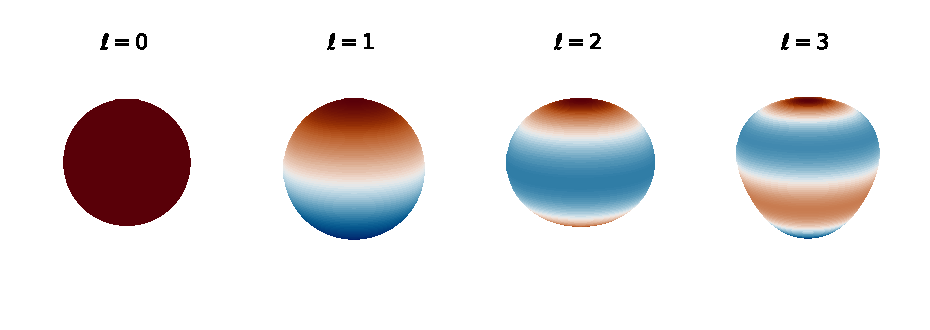
\includegraphics[trim={0 0.4in 0 0},clip]{figures/spherical_harmonics.pdf}
    \caption{Spherical harmonic oscillation modes for a few angular degrees ($l$) with azimuthal order \(m=0\). The colour-map represents the radial displacement at the surface, with \emph{red} and \emph{blue} corresponding to displacement inward and outward respectively. These regions oscillate in and out, with the white regions representing stationary nodes on the surface.}
    \label{fig:spherical-harmonics}
\end{figure}

Oscillations on the surface of a star can be approximated by spherical harmonic functions with angular degree \(l\) and azimuthal order \(m\). The angular degree is the number of nodes on the surface of the star. We show a representation of the surface spherical harmonics for the first four angular degrees in Figure \ref{fig:spherical-harmonics}. For each \(l\), there exists \(2l+1\) solutions with different azimuthal order (\(m\)) corresponding to the different orientations of the nodes over the spherical surface. Additionally, the oscillation modes have unique frequency solutions for different radial orders (\(n\)), proportional to the number of wave nodes radially throughout the star.

\begin{figure}[tb]
    \centering
    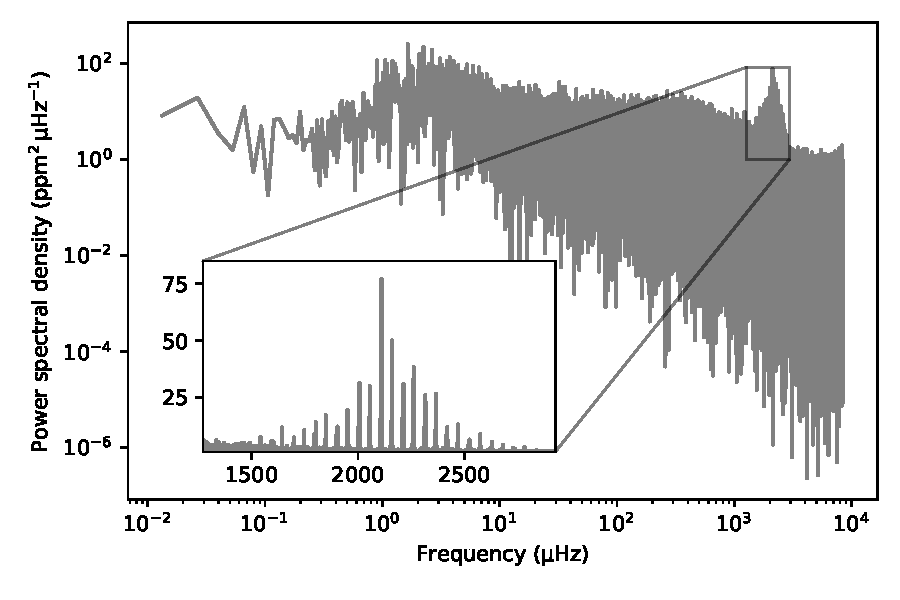
\includegraphics{figures/seismo-psd.pdf}
    \caption{The power spectral density of 16 Cyg A. The inset plot highlights the Gaussian-like power excess in the larger plot.}
    \label{fig:seismo-psd}
\end{figure}

In solar-like oscillators, p modes are stochastically excited by near-surface convection. Typically, the timescale of this process drives high-order modes in main sequence stars \needcite[\(n \sim 20\)]. We can identify these modes in a frequency-power spectrum derived from photometric or radial velocity time series observations. For instance, both stars in the 16 Cyg system are solar-like oscillators with similar properties to the Sun \needcite. Using 16 Cyg A as an example, we downloaded the power spectrum determined by the \emph{Kepler} Asteroseismic Science Operations Centre (KASOC) using \emph{Kepler} observations\footnote{\url{https://kasoc.phys.au.dk}}. Shown in Figure \ref{fig:seismo-psd}, the power spectrum of 16 Cyg A has a distinct power excess around \SI{2000}{\micro\hertz}. 

We call the location of the peak in power excess the `frequency at maximum power', \(\numax\). Dependent on near-surface conditions, \citet{Brown.Gilliland.ea1991} suggested \(\numax\) scales with the acoustic cut-off frequency --- the highest frequency at which acoustic waves can reflect near the stellar surface. Subsequently, \citet{Kjeldsen.Bedding1995} found that \(\numax \propto g\teff^{\,-1/2}\) where \(g\) and \(\teff\) are the near-surface gravitational field strength and temperature. The power excess also has a Gaussian-like shape around \(\numax\). We expect this shape to come from the distribution in convection timescale near the surface responsible for mode excitation \needcite.

Looking closely at the power excess in Figure \ref{fig:seismo-psd}, we can see a comb of approximately equally spaced peaks. Each peak corresponds to one or more oscillation modes, with its central frequency and shape providing information about the internal stellar structure. Naturally, higher frequency modes correspond to higher \(n\). However, the angular degree and azimuthal order are harder to identify. We saw in Figure \ref{fig:spherical-harmonics} how modes of higher \(l\) have more anti-nodes on the surface. Therefore, the overall effect of the oscillations cancel out when integrating over the observed surface. Consequentially, observed mode amplitude decreases with \(l\) when observing total stellar irradiance, leaving only \(l \lesssim 3\) detectable \needcite. With this assumption, we can assume the tallest peaks are \(l=0,1\), and the smaller peaks are \(l=2,3\), all modulated by the wider Gaussian-like envelope.

As an aside, the observed mode frequencies will split for different \(m\) via the Doppler effect in the case of a rotating star. Measuring this splitting can constrain the rotation rate of the star. This has lead to breakthrough studies into gyrochronology and\dots \citep[e.g.][]{Hall.Davies.ea2021}. However, we will hereafter consider the case of a slowly rotating, spherically symmetric star, such that solutions of different \(m\) are approximately the same frequency.

If we consider an acoustic wave in a one-dimensional homogeneous medium, then we would expect each mode of oscillation to be an integer multiple of the fundamental mode. While the case for a star is more complicated, we can also approximate the frequencies for different modes as a multiple of some characteristic frequency. \citet{Tassoul1980} found that the modes could be approximated by assuming the asymptotic limit where \(l/n \rightarrow 0\), giving the following expression \citep[cf.][]{Gough1986},
%
\begin{equation}
    \nu_{nl} \simeq \left(n + \frac{l}{2} + \varepsilon\right) \nu_0 + O(\nu_{nl}^{-1}), \label{eq:asy}
\end{equation}
%
where \(\varepsilon\) is some constant offset and \(O\) represents higher order terms. The characteristic frequency, \(\nu_0\), is the inverse of the acoustic diameter,
%
\begin{equation}
    \nu_0 = \left(2 \int_{0}^{R} \frac{\dd r}{c(r)}\right)^{-1},
\end{equation}
%
where \(c(r)\) is the sound speed as a function of radius, \(r\), and \(R\) is the stellar radius. Similarly to other variable stars, \citet{Ulrich1986} found that this characteristic frequency relates to the mean density by \(\nu_0 \propto \overline{\rho}^{\,1/2}\). While \(\nu_0\) is not directly detectable in solar-like oscillators, we can approximate it by taking the difference between consecutive modes of the same angular degree, \(\Delta\nu_{nl} = \nu_{nl} - \nu_{n-1\,l}\). Thus, Estimates of a global (or average) large frequency separation, \(\Delta\nu \simeq \nu_0\), can provide information about the density of a star, leading to independent constraint on its mass and radius.

\begin{figure}[tb]
    \centering
    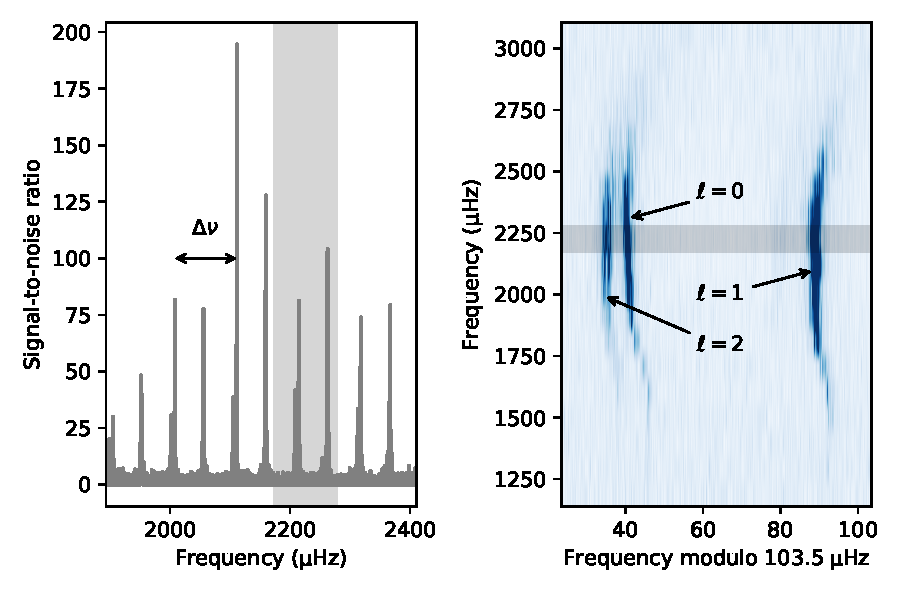
\includegraphics{figures/seismo-echelle.pdf}
    \caption{\emph{Left:} A section of the spectral signal-to-noise ratio (SNR) against frequency for 16 Cyg A. The large frequency spacing (\(\Delta\nu\)) between two radial modes is annotated with a double-headed arrow. The shaded region corresponds to a single row (also highlighted) in the echelle plot (\emph{right}). The echelle plot shows the spectral SNR such that a darker colour represents a higher SNR. Each row spans \SI{103.5}{\micro\hertz} and is stacked in order of frequency. The apparent ridges are labelled according to the angular degree (\(l\)) of the modes they represent.}
    \label{fig:seismo-echelle}
\end{figure}

The asymptotic expression helps us identify modes in a star. If the first term of Equation \ref{eq:asy} was exact, we would expect odd and even modes to be grouped together and separated by \(\dnu/2\). To see this, we revisit the power spectrum of 16 Cyg A, now with an estimate of the noise divided out. We can see the regular pattern predicted by Equation \ref{eq:asy} in the left panel of Figure \ref{fig:seismo-echelle}. Every other mode is approximately separated by \(\dnu\). To see this effect over the wider spectrum, we created an \emph{echelle} plot in the right panel. Folding the spectrum by an estimate of \(\dnu\) reveals a sequence of ridges corresponding to modes of different angular degree. Odd and even angular degree are grouped together, although do not lie on top of each other. The small difference between modes of different \(l\) is described by the higher order terms neglected from Equation \ref{eq:asy}. A faint ridge corresponding to \(l=3\) modes is also visible next to the \(l=1\) ridge. However, 16 Cyg A represents one of the highest signal-to-noise dwarf stars observed by \emph{Kepler}, so the \(l=3\) ridge is usually not visible. 

% Once we have identified a solar-like oscillator, what information is there to gain from asteroseismology? We have discussed how parameters \(\numax\) and \(\dnu\) scale with global stellar properties. Scaling these parameters with respect to the Sun, we can obtain relations for the radius and mass of the star,
% %
% \begin{align}
%     \left(\frac{R}{\si{\solarradius}}\right) &\simeq \left(\frac{\numax}{\numax_{,\odot}}\right) \left(\frac{\dnu}{\dnu_\odot}\right)^{-2} \left(\frac{\teff}{\teff_{,\odot}}\right)^{1/2},\\
%     \left(\frac{M}{\si{\soNonlarmass}}\right) &\simeq \left(\frac{\numax}{\numax_{,\odot}}\right)^3 \left(\frac{\dnu}{\dnu_\odot}\right)^{-4} \left(\frac{\teff}{\teff_{,\odot}}\right)^{3/2}.
% \end{align}
% %
% Using these relations directly can provide quick-look, independent mass and radius estimates \citep[e.g.][]{Pinsonneault.Elsworth.ea2018}.

% We can also use individual modes and compare with models. Worth noting the surface term here.

\todo{final pargraph rounding out section.}

\section{Modelling Stars the Bayesian Way}\label{sec:modelling-stars}

% The phrase `modelling stars' can be confusing. We often use it to describe the process of numerically simulating the physics of a star. Some examples of such simulations are one-dimensional stellar evolution codes (e.g. MESA) and three-dimensional hydrodynamical simulations \todo{e.g. other}. However, we also use the word `model' in probabilistic inference to refer to the process of generating predictions with some set of model parameters given some observed data \citep[e.g.][]{Hogg.Bovy.ea2010}. In this thesis, we prefer the phrase `modelling stars' to mean the entire process of inferring stellar parameters using a generative model. To model a given star, we may need to compute many stellar simulations, but the overall model compares these simulations to data in a probabilistic way. To avoid confusion where possible, we refer to numerical models of stars as either stellar simulations or evolutionary models.

\todo{Something about how astronomers want stellar masses and stuff. These help with uncovering the chemodynamical history of the milky way. Ages help find mergers. Also masses are good for exoplanets. }

In some cases, stellar parameters can be estimated directly from observables using empirical relationships. For example, mass-luminosity relation, or asteroseismic scaling relations.

Alternatively, we can compare the results of stellar evolutionary models to observed data. These models come from physical simulations which take inputs (e.g. the initial mass and metallicity) and output observable parameters (e.g. luminosity and effective temperature). For example, the software package `Modules for Experiments in Stellar Astrophysics' (MESA), originally developed by \citet{Paxton.Bildsten.ea2011}, is a one-dimensional stellar evolution code. Assuming spherical symmetry, MESA simulates the structure and evolution of a star along a one-dimensional radial slice. At its core, the code numerically solves a series of differential equations which govern the interior dynamics of the star \citep[see e.g.][]{Kippenhahn.Weigert.ea2013}.

With the advent of high-precision asteroseismology, we can also compare measurements of oscillation mode frequencies to simulations. For example, the GYRE code developed by \citet{Townsend.Teitler2013} uses the output of MESA to compute oscillation modes for a given \(n\) and \(l\). While the physics of p mode propagation in the star is relatively well-known \citep[see e.g.][]{Aerts.Christensen-Dalsgaard.ea2010}, our understanding of the atmospheric boundary conditions are not. As such, there is a known discrepancy between the simulated and observed p modes. The nature of this \citep{Ball.Gizon2014}.

There are a handful of existing methods for determining stellar parameters through comparison to one-dimensional evolutionary models. 

% With the advent of high-precision asteroseismology for many stars, astronomers have a plethora of observables to constrain physical models of stellar evolution. 

% A la carte modelling involves producing and optimising dedicated stellar models for a given star. Many parameters can be optimised this way, but it is slow.

% Grid-based modelling involves producing a large grid of stellar models and computing the likelihood across the grid. Some examples. Assumptions must be made on approximations of stellar physics such as helium and MLT. Also overshoot, diffusion, rotation, solar abundances and opacity tables.

Modelling stars the Bayesian way involves estimating the probability of stellar parameters (e.g. \(\theta = \text{mass, age}, \dots\)) given observations (\(y = \text{luminosity, effective temperature}\)). We can do this starting with Bayes' theorem for the \emph{posterior} probability density,
%
\begin{equation}
    p(\theta \mid y) = \frac{p(y \mid \theta)\,p(\theta)}{p(y)},
\end{equation}
%
where \(p(y \mid \theta)\) is the likelihood, \(p(\theta)\) is the \emph{prior}, and \(p(y)\) is the \emph{evidence}. The prior encodes our expectation for \(\theta\). If our data are bad, then the prior dominates and we return our current belief. However, if the data are good enough, then they have more influence on the posterior and our belief is updated. As a result, we can use the Bayesian methodology to systematically update our beliefs. 

Marginalised probability distribution,
%
\begin{equation}
    p(\theta_i \mid y) = \int_{\vect{\theta}_{j \neq i}} p(\vect{\theta} \mid y) \dd \vect{\theta}_{j \neq i}
\end{equation}
%

In practice, our likelihood depends on our choice of model. The model is the function which maps \(\theta\) to observable parameters, \(\tilde{y} = f(\theta)\). When modelling stars, this function is rarely analytical. Therefore, the posterior distribution must be estimated using a numerical method. Some methods include Markov Chain Monte Carlo and nested sampling \needcite. Typically, these methods involve multiple calls to \(f\) with different values of \(\theta\). This presents a problem when using stellar evolutionary models like MESA. These models are slow to evaluate and computationally expensive.

% For example, if we used MESA as our model, \(\theta\) would represent inputs to the code. 

With some observables, these methods are good enough. Systematics within the uncertainty budget.

With asteroseismology providing more precise observables, the systematics in stellar models have been highlighted. With no observed counterpart, stellar age has the most uncertainty.

Next section deals with the scalability.

% Stellar model-based properties are often found on a star-by-star basis. For example, minimising the likelihood of observables across a grid of 1D evolutionary models. While this approach can be fast and effective, it fails to weight the likelihood by our prior beliefs. For example, the universe is 14 billion years old, yet some stellar models return ages greater than this. This is usually attributed to systematic bias in our models, but what if we can parametrise this bias? Then, our prior on age can inform us of where our bias lies. The statistical framework for incorporating prior beliefs is known as Bayesian inference. This has been applied recently to stellar parameters (BASTA). However, we can do better by including prior beliefs on the distribution of a population of stars.

\section[Modelling Stars with Asteroseismology]{Modelling Many Stars with Asteroseismology}

Large scale surveys like \emph{Kepler} and \emph{TESS} have allowed for asteroseismology with many stars. This has allowed astronomers to study regions of the HR diagram in more detail, from main sequence dwarf stars to helium burning red clump stars. While \emph{TESS} is an all-sky survey, it's short baseline of a few months for many stars limits the mode identification and precision with asteroseismology. On the other hand, \emph{Kepler} looked at a single patch of the sky for several years. Currently, \emph{Kepler} still provides the best samples of solar-like oscillators. Therefore, we focus on solar-like oscillators observed by \emph{Kepler} in this thesis, with the potential to apply our methods to future missions with longer baselines.

The majority of solar-like oscillations found with \emph{Kepler} are red giant stars. These have been used for galactic archaeology coupled with Gaia. However, stars spend most of their time on the main sequence. 

We focus on dwarf and subgiant solar-like oscillators partly because it makes sense to start at the beginning of a star's life but also because this is the region where the most planet hosts have been discovered.

\begin{figure}
    \centering
    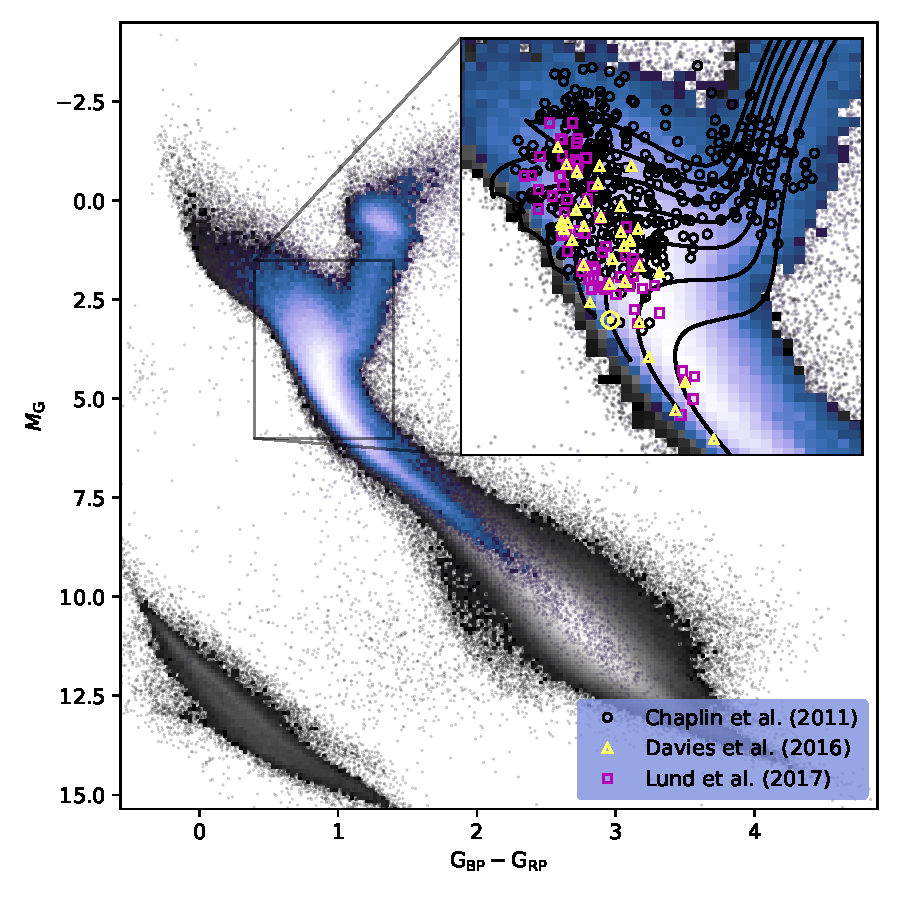
\includegraphics{figures/hr-diagram.pdf}
    \caption[Colour-magnitude diagram highlighting the region occupied by dwarf and subgiant solar-like oscillators.]{Colour-magnitude diagram highlighting the region occupied by solar-like oscillators. The data are \emph{Gaia} green, blue, and red band magnitudes given by G, G\textsubscript{BP}, and G\textsubscript{RP} respectively. The absolute magnitude (\(M_\mathrm{G}\)) is calculated from \emph{Gaia} magnitude and parallax neglecting extinction. The \emph{greyscale} 2D histogram shows the density of \emph{Gaia} DR3 targets with parallax \(>\SI{5}{\milli\aarcsec}\) (distance \(\lesssim\SI{200}{\parsec}\)). The \emph{coloured} 2D histogram shows the density of all \emph{Kepler} targets in \emph{Gaia} DR3. MIST stellar evolutionary tracks at solar metallicity are given by the \emph{black lines} for \SIrange{0.8}{1.4}{\solarmass} in steps of \SI{0.1}{\solarmass}. The points in the inset axes correspond to \emph{Kepler} solar-like oscillators with references given in the legend, where \emph{yellow} represents confirmed planet hosts. The Sun is given by the `\(\odot\)' symbol.}
    \label{fig:hr-diagram}
\end{figure}

We show a colour-magnitude diagram for context in Figure \ref{fig:hr-diagram}. Using magnitudes and parallaxes from \emph{Gaia} Data Release 3 \citep[DR3;][]{GaiaCollaboration.Vallenari.ea2022}. We see the Kepler-Gaia cross-match\footnote{\url{https://gaia-kepler.fun}}. The densest region lies in the low- to intermediate-mass main sequence (\SIrange{0.8}{1.2}{\solarmass}).

These targets have since been studied extensively. Give some examples.

The modes were identified for a sample of 33 exoplanet host stars by \citet{Davies.Aguirre.ea2016} and modelled by \citet{SilvaAguirre.Davies.ea2015}. With most exoplanet hosts being in their main sequence phase \needcite...

The so-called LEGACY sample modes identified by \citet{Lund.SilvaAguirre.ea2017} modelled by \citet{SilvaAguirre.Lund.ea2017}.

Then the APOKASC project, combining asteroseismology with APOGEE spectroscopy extended the modelling to around 400 dwarf and subgaints \citep{Serenelli.Johnson.ea2017}. Between then and now, there has not been a similar sized catalogue of dwarf stars from K2 and TESS.

However, there have been many sources of systematic uncertainty. Many assumptions were made in the modelling of this sample of stars. It is a perfect test case for new modelling methods. Then the plan is to apply these to future missions like Plato and Nancy Grace Roman.

In the next chapter, we introduce hierarchical Bayesian models. We explore a simple HBM in the context of astronomy and show how it can improve the estimates of stellar parameters.

Following that, we present a hierarchical model of helium enrichment on a population of dwarf and subgiant stars observed by \emph{Kepler} in Chapter \ref{}. While such a method improves upon and tackles bias in our choice of helium enrichment, there is more helium abundance information to be gained from asteroseismology.

Finally, in Chapter \ref{}, we explore signatures of helium abundance in the oscillation modes of stars. We present a new method for characterising these glitches.
